\documentclass[11pt,a4paper]{article}
\usepackage[utf8]{inputenc}
\usepackage[T1]{fontenc}
\usepackage{amsmath,amssymb,amsthm}
\usepackage[a4paper,margin=2.4cm]{geometry}
\usepackage{booktabs}
\usepackage{xcolor}
\usepackage{enumitem}
\usepackage{parskip}
\usepackage{titlesec}
\usepackage{hyperref}
\usepackage{tikz}

\titleformat{\section}{\large\bfseries}{\thesection}{0.6em}{}
\titleformat{\subsection}{\normalsize\bfseries}{\thesubsection}{0.6em}{}
\hypersetup{colorlinks=true,linkcolor=blue,citecolor=blue,urlcolor=blue}

\definecolor{cred}{HTML}{cf222e}
\definecolor{cgreen}{HTML}{2ea043}
\definecolor{cblue}{HTML}{0969da}

\newcommand{\Vs}{\mathcal{V}}
\newcommand{\Ws}{\mathcal{W}}
\newcommand{\Id}{\mathrm{Id}}
\newcommand{\ran}{\operatorname{range}}
\newcommand{\rk}{\operatorname{rank}}

\title{Multi-level dynamics on a multiresolution grid:\\
\large the level ladder is \emph{one-sided}, and what to do about it}
\author{Internal note, connectome-gnn project}
\date{2026-08-29}

\begin{document}
\maketitle

\begin{quote}
\textbf{Short answer.} We want to learn a dynamics model whose levels split the work by
scale: coarse levels owning large, slow structure and fine levels owning small, fast
structure. Building the levels out of a multiresolution grid gives us \emph{half} of that
for free. A coarse level genuinely cannot express fine structure --- that half is a hard,
structural guarantee. But the converse does not hold: a fine level can reproduce coarse
structure perfectly well, so nothing stops the finest level from swallowing the entire
model and leaving the hierarchy empty. The ladder of spaces is nested, not orthogonal;
it is a \emph{one-sided} constraint. The repair is to make each level \emph{band-pass}
rather than \emph{low-pass}, by subtracting off whatever the next coarser level could
already have said. The same argument, word for word, applies on the time axis, and it
applies again --- with the grid replaced by a hierarchy of groups of neurons --- when
the data lives on a connectivity matrix $W_{ij}$ rather than in space.
\end{quote}

\tableofcontents

\section{What we are building, in words}

We have two pieces already.

The first is a \emph{multiresolution hash encoding} (Instant-NGP, M\"uller et al.\ 2022,
arXiv:2201.05989; our implementation is \texttt{ngp-demo/ngp/hashgrid.py}). It stores a
learnable feature vector at the vertices of a stack of grids, from a coarse grid to a fine
one, and answers a query at a point by reading the corners of the cell containing that
point at every grid and interpolating. Because the fine grids have more vertices than the
table has rows, several vertices share a row; those \emph{collisions} are the mechanism by
which the encoding decides, on its own, which parts of the domain deserve fine detail. When
two samples share a row their gradients add, and the sample that matters more to the loss
dominates the sum.

The second is a \emph{graph neural network} that predicts a rate of change from a state and
a per-unit embedding (\texttt{connectome-gnn}). Today that embedding is a free parameter,
one independent vector per neuron (\texttt{drosophila\_cx\_task\_gnn.py:459}).

The proposal is to fuse them: let the encoding supply both the state and the embedding, let
one small network per level predict a rate of change, and add the levels up. The hoped-for
payoff is that the dynamics model inherits the encoding's automatic allocation ---
\emph{fine levels end up owning small regions with fast activity, coarse levels large
regions with slow activity} --- without anyone hand-designing the hierarchy.

This note asks whether that actually follows. The answer is: half of it does, and the
missing half has a clean fix.

\medskip
\noindent\textbf{Notation, stated once.} We write $r=(x,y,z)$ for a position and $t$ for
time, and reserve $u$ for the \emph{state} being modelled (a voltage, a fluorescence, a
concentration) so that it is never confused with the coordinate $x$. A dot denotes the time
derivative, so $\dot u$ is the rate of change we want to predict. Levels are indexed by
$\ell = 0,1,\dots,L$, with $\ell=0$ the \emph{coarsest} and $\ell=L$ the \emph{finest}.

\section{Part I --- Volumetric data: a state sampled over space and time}
\label{sec:spatial}

Start with the easy case. The data is a state $u(r,t)$ observed on a volume $\Omega
\subset \mathbb{R}^3$ over a time interval $[0,T]$ --- a light-sheet recording, say. There
is no connectivity matrix yet; the only structure is that nearby points are neighbours.

\subsection{The three operators}

Level $\ell$ owns a regular grid $G_\ell$ with $n_\ell$ vertices and spacing $h_\ell$. The
spacings shrink geometrically,
\begin{equation}
h_\ell \;=\; h_0\, b^{-\ell},
\qquad b>1 ,
\label{eq:ladder}
\end{equation}
where $b$ is the per-level scale factor (\texttt{per\_level\_scale}, default $1.5$ in our
code, meaning \emph{each level's cells are $1.5\times$ smaller per axis than the level
above}).

\paragraph{Prolongation $I_\ell$ --- going from grid values up to the full domain.} This is
exactly the encoding's own interpolation. Given one number (or one vector) $c_v$ per
level-$\ell$ vertex $v$, it produces a function of position by reading the $2^3=8$ corners
of the cell containing $r$ and weighting them:
\begin{equation}
(I_\ell c)(r) \;=\; \sum_{v \,\in\, \mathrm{corners}_\ell(r)} w_\ell(v,r)\, c_v ,
\qquad
\sum_{v} w_\ell(v,r) = 1 ,
\label{eq:prolong}
\end{equation}
with $w_\ell$ the multilinear weights (or their smoothstep variant $3w^2-2w^3$, which our
implementation offers per axis and which is what you need if second derivatives are taken
through the encoding).

\paragraph{Restriction $P_\ell$ --- going from the full domain down to grid values.} The
simplest choice is evaluation at the vertices,
\begin{equation}
(P_\ell f)_v \;=\; f(r_v) ,
\label{eq:restrict}
\end{equation}
which has the property we will lean on repeatedly:
\begin{equation}
P_\ell I_\ell \;=\; \Id_{n_\ell}
\qquad\text{(interpolation reproduces the values it was built from).}
\label{eq:PI}
\end{equation}
\textbf{Property \eqref{eq:PI} is not a technicality, and the cheap restriction does not
have it.} When the data is scattered rather than sitting on the vertices, the tempting
choice is the encoding's own backward scatter, the mass-normalised adjoint
$P_\ell = D_\ell^{-1} I_\ell^{\!\top}$ with $D_\ell = \mathrm{diag}(I_\ell^{\!\top}\mathbf{1})$,
because it costs one scatter and reuses machinery that is already there. It is \emph{not} a
left inverse, and the whole of \S\ref{sec:fix} collapses without one. Measured on a
five-level dyadic ladder in one dimension:

\begin{center}
\begin{tabular}{@{}lccc@{}}
\toprule
\textbf{choice of $P_\ell$} & $\max\|P_\ell I_\ell - \Id\|$ & $\|I_\ell P_\ell\|_2$
  & \textbf{detail dimensions $\dim\Ws_\ell$} \\
\midrule
$I_\ell^{+}$, least squares      & $2.4\times10^{-15}$ & $1$ & $5,4,8,16,32$ \quad(exactly $n_\ell - n_{\ell-1}$) \\
$D_\ell^{-1}I_\ell^{\!\top}$, normalised adjoint & $0.33$ & $1$ & $5,8,16,32,64$ \quad($=n_\ell-1$) \\
$I_\ell^{\!\top}$, raw adjoint   & $3.4\times10^{2}$ & up to $475$ & $5,9,17,33,65$ \quad($=n_\ell$) \\
\bottomrule
\end{tabular}
\end{center}

\noindent
Only the least-squares restriction telescopes. The normalised adjoint produces detail spaces
of dimension $n_\ell - 1$: it removes the constant mode and \emph{nothing else}, so the
band-pass degenerates into an expensive way of subtracting a mean. The raw adjoint removes
nothing at all and amplifies the coarse content by up to $475\times$ \emph{its own
amplitude}, which would invert and blow up exactly the structure it was meant to subtract.
So $P_\ell$ must solve the level-$\ell$ Gram system, not scatter --- see the cost note in
\S\ref{sec:fix}.

\paragraph{The level operator $\mathrm{GNN}_\ell$.} A small network living \emph{on the
level-$\ell$ grid}: it takes the restricted state and the level's embedding at every
vertex, passes messages between neighbouring vertices, and emits one predicted rate of
change per vertex. It reads only level-$\ell$ things and writes only level-$\ell$ things.

\subsection{The model}

Putting the three together, the proposed model is
\begin{equation}
\boxed{\;
\dot u^{*}(r,t) \;=\; \sum_{\ell=0}^{L} I_\ell\Big[\,
   \mathrm{GNN}_\ell\big(\, P_\ell u,\; a_\ell \,\big)
\Big](r,t)
\;}
\label{eq:model-naive}
\end{equation}
where $a_\ell$ is the level-$\ell$ slice of the shared hash table --- the multiresolution
embedding, which is the novel object we are after. It is trained with two terms, one that
makes the encoding reproduce the observations and one that makes the summed operator
reproduce the dynamics:
\begin{equation}
\mathcal{L} \;=\;
\underbrace{\big\| u' - u \big\|^2}_{\text{data fit}}
\;+\;
\lambda \underbrace{\big\| \dot u^{*} - \dot u \big\|^2}_{\text{model fit}} .
\label{eq:loss}
\end{equation}

\subsection{The spaces, and the nesting}

Everything below is about \emph{what each level can possibly say}. Define
\begin{equation}
\Vs_\ell \;:=\; \ran(I_\ell)
\;=\;\{\, \text{functions that are interpolations of level-$\ell$ vertex values} \,\},
\qquad \dim \Vs_\ell = n_\ell .
\label{eq:Vspace}
\end{equation}
Level $\ell$'s contribution to \eqref{eq:model-naive} lies in $\Vs_\ell$ and nowhere else,
whatever the network inside does. That is the whole point of putting the network on the
grid: the bandwidth is imposed by the \emph{geometry}, not by the network.

The essential structural fact is that these spaces are \emph{nested}:
\begin{equation}
\Vs_0 \;\subset\; \Vs_1 \;\subset\; \cdots \;\subset\; \Vs_L .
\label{eq:nested}
\end{equation}
A function that is multilinear on the coarse cells is still multilinear on each fine cell,
so anything the coarse grid can say, the fine grid can say too.

\begin{center}
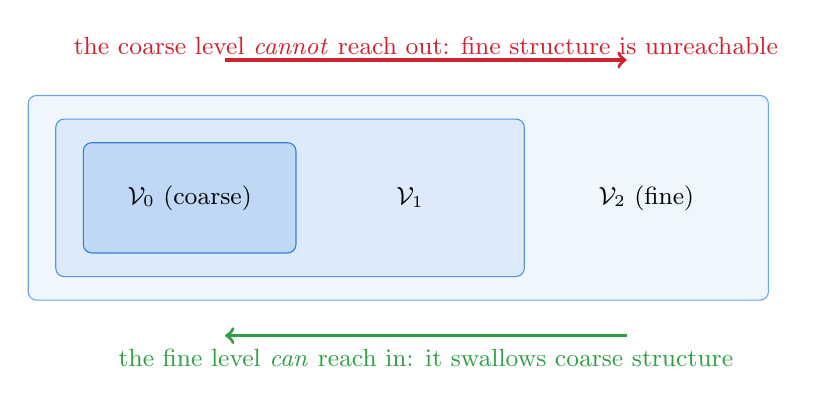
\begin{tikzpicture}[scale=1.0]
  \draw[rounded corners=3pt, fill=cblue!6, draw=cblue!60]
        (0,0) rectangle (9.4,2.6);
  \draw[rounded corners=3pt, fill=cblue!14, draw=cblue!70]
        (0.35,0.3) rectangle (6.3,2.3);
  \draw[rounded corners=3pt, fill=cblue!26, draw=cblue!85]
        (0.7,0.6) rectangle (3.4,2.0);
  \node at (2.05,1.3) {\small $\Vs_0$ (coarse)};
  \node at (4.85,1.3) {\small $\Vs_1$};
  \node at (7.85,1.3) {\small $\Vs_2$ (fine)};
  \draw[->, very thick, cgreen] (7.6,-0.45) -- (2.5,-0.45);
  \node[below, cgreen] at (5.05,-0.5)
        {\small the fine level \emph{can} reach in: it swallows coarse structure};
  \draw[->, very thick, cred] (2.5,3.05) -- (7.6,3.05);
  \node[above, cred] at (5.05,3.0)
        {\small the coarse level \emph{cannot} reach out: fine structure is unreachable};
\end{tikzpicture}
\end{center}

\subsection{The one-sidedness, stated precisely}
\label{sec:onesided}

This is the heart of the note. The constraint that the grid gives us runs in one direction
only.

\paragraph{Direction that holds: coarse cannot reach fine.} Let $\Pi_\ell$ be the
orthogonal projector onto $\Vs_\ell$. For any target rate of change $f$,
\begin{equation}
\min_{c} \; \big\| I_\ell c - f \big\|
\;=\; \big\| (\Id - \Pi_\ell) f \big\|
\;\geq\; \big\| f_{\,>\,1/2h_\ell} \big\| ,
\label{eq:coarse-cannot}
\end{equation}
where $f_{\,>\,1/2h_\ell}$ is the part of $f$ whose spatial frequency exceeds the
level-$\ell$ Nyquist frequency, one half cycle per cell. \textbf{No choice of network
weights lets level $\ell$ produce structure finer than its own cell.} This bound is
structural, it involves no assumption about training, and it is why the construction is
attractive in the first place.

\paragraph{Direction that fails: fine can swallow coarse.} By the nesting
\eqref{eq:nested}, for any coarse coefficient vector $\delta$ on level $\ell-1$ there is a
fine coefficient vector on level $\ell$ producing \emph{exactly} the same function, namely
$P_\ell I_{\ell-1}\delta$. So the following move changes nothing at all in the model's
output:
\begin{equation}
c_{\ell-1} \;\longmapsto\; c_{\ell-1} - \delta ,
\qquad
c_{\ell} \;\longmapsto\; c_{\ell} + P_\ell I_{\ell-1}\,\delta ,
\qquad\text{for any }\delta \in \mathbb{R}^{n_{\ell-1}} .
\label{eq:gauge}
\end{equation}
Verify it directly: the change in the sum is $-I_{\ell-1}\delta + I_\ell P_\ell
I_{\ell-1}\delta = 0$, since $I_\ell P_\ell$ acts as the identity on $\Vs_{\ell-1} \subset
\Vs_\ell$. This is a \emph{gauge freedom}: a whole family of level assignments produces
byte-identical predictions and byte-identical loss.

\paragraph{How big is the ambiguity?} Stack the prolongations into one operator
$\mathbf{I} = [\,I_0 \; I_1 \;\cdots\; I_L\,]$ acting on all level coefficients at once.
Its range is $\Vs_L$ (by nesting, the sum of the spaces is the largest one), so its null
space has dimension
\begin{equation}
\dim \ker \mathbf{I}
\;=\; \sum_{\ell=0}^{L} n_\ell \;-\; n_L
\;=\; \sum_{\ell=0}^{L-1} n_\ell .
\label{eq:nulldim}
\end{equation}
With vertex counts growing geometrically, $n_\ell = n_0\, g^{\ell}$ where $g = b^{D}$ is
the per-level growth factor in \emph{number of vertices} for a $D$-dimensional grid, the
unidentifiable fraction is
\begin{equation}
\frac{\dim \ker \mathbf{I}}{\sum_{\ell} n_\ell}
\;=\; \frac{g^{L}-1}{g^{L+1}-1}
\;\xrightarrow[\;L \text{ large}\;]{}\; \frac{1}{g}
\;=\; b^{-D} .
\label{eq:nullfrac}
\end{equation}
At our default per-level scale $b=1.5$: in three space dimensions $g = 1.5^3 = 3.375$, so
\textbf{about $30\%$ of all level coefficients are pure gauge} --- they move structure
between levels without changing a single predicted value. Adding the time axis ($D=4$,
$g=5.06$) softens it to $20\%$; on the \emph{time axis alone} ($D=1$, $g=1.5$) it is
$67\%$, two thirds. The temporal ladder is by far the worst offender, which is the subject
of \S\ref{sec:time}.

\paragraph{Two honest caveats.}
\begin{enumerate}[leftmargin=1.4em,itemsep=2pt]
\item \emph{The nesting is only exact for a dyadic ladder.} With $b=2$ each fine grid is a
refinement of the coarse one and \eqref{eq:nested} is exact. At $b=1.5$ the fine grid is
not a refinement, so the containment holds only up to interpolation error, of order
$h_\ell^2$ times the curvature of the coarse function. This does \emph{not} rescue the
situation. A near-null direction is worse than an exact one: gradient descent does not stop
on it, it drifts along it slowly, so the level assignment keeps changing during training
without the loss ever objecting.
\item \emph{Hashing perturbs the nesting in an uncontrolled way.} Once a level has more
vertices than the table has rows, several vertices are forced to share a row, so the
level's effective space has rank at most the table size $T$ and is no longer a clean
superset of the coarser space. This partially breaks the swallowing --- accidentally, and
in a scattered, random pattern that also damages the fine level's ability to represent
legitimate fine detail. It is not a substitute for the fix below.
\end{enumerate}

\subsection{Why the one-sidedness matters in practice}

Three consequences, in increasing order of seriousness.

\begin{enumerate}[leftmargin=1.4em,itemsep=3pt]
\item \textbf{Any hierarchy you read off the trained model is an artefact.} If you plot
``how much does level $\ell$ contribute'', you are plotting a quantity that the loss does
not determine. Two runs from different seeds can produce identical predictions and
completely different level profiles.

\item \textbf{The automatic allocation story does not go through.} Instant-NGP's argument
is about \emph{which samples win a shared table row}, and that argument is intact. But it
says nothing about \emph{which level a piece of structure ends up on}, because moving
structure between levels costs nothing. There is no pressure to be coarse.

\item \textbf{The collapse is toward the worst level.} The finest level has the most
parameters and, being hashed, the most collisions. Gradient descent has no reason to prefer
the coarse levels, and the fine level can express everything, so the likely outcome is that
the model uses the fine level for the slow global drift as well --- spending its scarcest,
most contended table rows on the structure that needed them least.
\end{enumerate}

\noindent
This is not only a prediction. Our own encoding repository carries a standing asserting test,
\texttt{ngp-demo/tests/level\_specialisation.py}, which measures how much each level
contributes to two halves of a signal that differ in scale, and records that the levels do
\emph{not} specialise: the contribution ratio spans $0.58$ to $1.14$ across levels running
from $8$ to $1407$ cells per axis, a spread of only $2.0\times$, under an assertion that the
spread stays below $5\times$. A ladder that had genuinely divided the work by scale would
show a spread of orders of magnitude, not a factor of two.

\subsection{The fix: make every level band-pass}
\label{sec:fix}

Subtract off whatever the next coarser level could already have said. Two operators, and it
matters which is which. First, the projector \emph{onto} the coarse space,
\begin{equation}
R_{\ell} \;:=\; I_{\ell} P_{\ell} ,
\qquad R_{-1} := 0 ,
\label{eq:R}
\end{equation}
which really is a projector, since $R_\ell^2 = I_\ell (P_\ell I_\ell) P_\ell = I_\ell
P_\ell = R_\ell$ by \eqref{eq:PI}. It is oblique rather than orthogonal, because $I_\ell$ is
an interpolation and not an isometry. Second, and this is the one that does the work, the
\emph{band-pass} operator that \emph{removes} everything already representable at level
$\ell-1$:
\begin{equation}
Q_{\ell} \;:=\; \Id - R_{\ell-1} \;=\; \Id - I_{\ell-1}P_{\ell-1} ,
\qquad Q_{0} := \Id .
\label{eq:Q}
\end{equation}
The corrected model is then
\begin{equation}
\boxed{\;
\dot u^{*} \;=\; \sum_{\ell=0}^{L}
Q_\ell\, I_\ell
\Big[\, \mathrm{GNN}_\ell\big(P_\ell u,\; a_\ell\big) \Big]
\;}
\label{eq:model-bandpass}
\end{equation}
This is a Laplacian pyramid, or equivalently a coarse-plus-residual decomposition: level
$\ell$'s contribution now lives in the \emph{detail space}
\begin{equation}
\Ws_\ell \;:=\; \Vs_\ell \ominus \Vs_{\ell-1}
\;=\; Q_\ell \Vs_\ell
\;=\; \Vs_\ell \cap \ker P_{\ell-1} ,
\qquad
\Ws_0 = \Vs_0 ,
\qquad \dim \Ws_\ell = n_\ell - n_{\ell-1} ,
\label{eq:Wspace}
\end{equation}
where $\ominus$ denotes the complement of $\Vs_{\ell-1}$ inside $\Vs_\ell$ taken along
$\ker P_{\ell-1}$ --- an \emph{oblique} complement, determined by the choice of restriction
$P_{\ell-1}$, which reduces to the orthogonal complement exactly when $P_{\ell-1}$ is the
orthogonal projection. The detail spaces are independent, giving a direct-sum decomposition
\begin{equation}
\Vs_L \;=\; \Ws_0 \oplus \Ws_1 \oplus \cdots \oplus \Ws_L .
\label{eq:directsum}
\end{equation}

\paragraph{What this buys, precisely --- and what it does not.} The decomposition of the
\emph{output} is now unique: given the predicted $\dot u^{*}$, each level's contribution is
determined, because a direct sum has no gauge freedom. The move \eqref{eq:gauge} is dead ---
a coarse function $\delta$ is annihilated by $Q_\ell$ and simply does not reach the output
from level $\ell$.

Two things this does \emph{not} buy, and both matter. First, it removes no ambiguity from
the \emph{parameters}: a per-level kernel of dimension $n_{\ell-1}$ survives at every level,
so the total nullity is unchanged. That redundancy is benign in the sense that it maps to
zero rather than redistributing structure --- and it can be removed entirely by
parameterising $c_\ell$ on $\Ws_\ell$ directly, at $n_\ell - n_{\ell-1}$ coefficients
instead of $n_\ell$ --- but anyone counting free directions will find exactly as many as
before. Second, and more seriously:

\begin{quote}
\textbf{The repair works only on an exactly nested ladder, and the default ladder is not
nested.} Everything in \S\ref{sec:fix} rests on $\Vs_{\ell-1}\subset\Vs_\ell$, and that
containment is exact only when each grid refines the one above it --- $b=2$. At the default
$b=1.5$ the fine grid is \emph{not} a refinement of the coarse one, $Q_\ell$ fails to
annihilate the part of $\Vs_{\ell-1}$ that lies outside $\Vs_\ell$, the detail spaces stop
being independent, and the uniqueness argument collapses.
\end{quote}

\noindent
This is measurable, and it was measured. On a one-dimensional ladder of five levels with an
exact left inverse $P_\ell = I_\ell^{+}$, evaluated on $4097$ query points:

\begin{center}
\begin{tabular}{@{}lcccc@{}}
\toprule
\textbf{ladder} & \textbf{nesting violation} & \textbf{nullity} & $\sum_\ell \dim\Ws_\ell$
  \textbf{vs.\ rank of span} & \textbf{unique?} \\
\midrule
$b=1.5$ (the default) & $0.23$ & $31 \to 31$ & $86$ vs.\ $79$ & no \\
$b=1.6$               & $0.22$ & $26 \to 26$ & $123$ vs.\ $105$ & no \\
$b=2.0$ (dyadic)      & $2.2\times10^{-15}$ & $64 \to 64$ & $65$ vs.\ $65$ & \textbf{yes} \\
\bottomrule
\end{tabular}
\end{center}

\noindent
The nesting violation is
$\max\big\|(\Id - I_\ell P_\ell)\,I_{\ell-1}\big\|$, \emph{the largest amount by which a
level-$(\ell-1)$ function fails to be representable at level $\ell$, as a fraction of that
function's own amplitude}. At $b=1.5$ it is $0.23$ --- almost a quarter of the coarse
function escapes the fine space, which is not a rounding error. The last column is the test
that matters: whether the sum of the detail-space dimensions equals the rank of their span,
which is exactly the condition for the per-level contributions to be recoverable from the
output. It holds at $b=2$ and fails otherwise. Note also that the nullity column is
unchanged in every row, confirming that the repair acts on the decomposition, never on the
parameter count.

\paragraph{Three prerequisites, all violated by the module defaults.} ``Set
\texttt{per\_level\_scale = 2}'' is necessary and not sufficient. The nesting the repair
needs has three separate requirements, each of which was measured and each of which the
current configuration fails.

\begin{enumerate}[leftmargin=1.6em,itemsep=3pt]
\item \textbf{Integer scale \emph{and} per-axis resolutions that divide.} Resolutions are
computed as $\mathrm{int}(\mathrm{round}(\mathrm{base}\times\mathrm{scale}^\ell))$
independently per axis, so a non-integer \emph{base} breaks divisibility even at scale $2$:
a base of $1.301$ gives the chain $3\to5$, not $3\to6$. A plausible micron-isotropic ladder
with bases $(2.000, 1.301, 0.699)$ fails $5$ of $18$ axis-pairs at scale $2$, and $29$ of
$33$ at scale $1.45$. \emph{Integer} per-axis bases fix it: $(8,5,3)$ at scale $2$ passes
$15$ of $15$ axis-pairs while staying isotropic in microns to within $11\%$ at every level
over an $830\times540\times290\,\mu$m field of view.
\item \textbf{Linear interpolation on every band-passed axis.} Smoothstep spaces are not
nested even at integer scale --- $11$ to $20\%$ \emph{of each coarse basis function} lies
outside the finer space --- because $3w^2-2w^3$ forces zero slope at every fine node. You
cannot have a wavelet ladder and a $C^1$ encoding on the same axis. If a Laplacian through
the encoding is needed, put smoothstep on a \emph{separate} encoder.
\item \textbf{$P_\ell$ must be a true left inverse}, per the table in \S\ref{sec:spatial}.
\end{enumerate}

\paragraph{And the cost is not the one the cheap recipe suggests.} Computing $I_\ell^{+}$ by
a few damped-Jacobi sweeps is the textbook trick, and it is a \emph{uniform-sampling} number.
On a realistic clustered geometry --- $13{,}700$ cells in about $30$ anisotropic nuclei
inside a brain-like shell, where $67\%$ of the finest level's nodes touch no cell at all ---
the fraction of each level's block Frobenius norm still left inside the coarse space was
measured at $0.966 / 0.784 / 0.700$ for levels $1/2/3$ with no lifting, $0.820 / 0.385 /
0.339$ after $8$ damped-Jacobi sweeps, and $0.331 / 0.096 / 0.191$ even after $128$ sweeps.
Sixty-four mass-preconditioned conjugate-gradient iterations \emph{restricted to occupied
nodes} give $3.4\times10^{-6} / 4.1\times10^{-3} / 7.0\times10^{-3}$. So: prune nodes whose
mass $d_\ell = I_\ell^{\!\top}\mathbf{1}$ is below a meaningful threshold --- at $10^{-8}$
the pruned Gram still has condition number $1.1\times10^{17}$ on clustered cells against
$63$ on uniform ones --- add a Tikhonov term $\varepsilon\,\mathrm{diag}(d_\ell)$ with
$\varepsilon = 10^{-4}$, and use a Krylov solver or a sparse Cholesky, not Jacobi. Keep the
density information by passing $d_\ell$ to the network as an extra input channel; never
leave it inside the projector.

\paragraph{The fallback if the ladder cannot be made nested.} Keep the plain sum
\eqref{eq:model-naive} and add an explicit penalty
$\lambda_{\mathrm{band}}\sum_{\ell\geq1}\big\|\Pi_{\ell-1}\,I_\ell\,c_\ell\big\|^2$ on the
\emph{output} of each level, with $\Pi_{\ell-1}$ the orthogonal projector onto $\Vs_{\ell-1}$
built on a \emph{fixed} reference query set and $\lambda_{\mathrm{band}} = 0.1$. That buys
leakage that is small rather than exactly zero, and it does not require nesting. The fixed
reference set is not optional: computed per minibatch, the projector silently annihilates the
fine levels --- at $1000$ samples against $4010$ table rows the finest level's dimension was
measured to collapse to $1$.

\paragraph{What this costs.} One extra restriction and one extra prolongation per level per
forward pass. Both are the operations the encoding already performs, so the cost is a small
constant factor on an operation that is not the bottleneck. There is no penalty weight to
tune, because the constraint is imposed by construction rather than by a regulariser.

\paragraph{The worry, and why it is misplaced.} One might fear that decreeing the hierarchy
destroys the automatic allocation we wanted in the first place. It does not, because the
two mechanisms act on different axes:

\begin{center}
\begin{tabular}{@{}lll@{}}
\toprule
& \textbf{acts across levels} & \textbf{acts within a level} \\
\midrule
mechanism & band-pass projection $Q_\ell$ & scarce capacity: fewer rows than cells \\
decides & \emph{which scale} owns a structure & \emph{which regions} get the rows \\
gives & identifiability & automatic allocation \\
imposed by & construction & training \\
\bottomrule
\end{tabular}
\end{center}

\noindent
Allocation was never the across-level degree of freedom; it was always the within-level
competition for scarce capacity. The band-pass removes only the redundancy, and leaves the
economy untouched.

\paragraph{A correction to the motivation: the sharing comes from quantisation, not from
collisions.} It is tempting to name the within-level mechanism ``hash collisions'', since
that is the mechanism Instant-NGP's paper describes. On our geometry that is the wrong end
of the ladder. Measured on the zebrafish soma positions (71{,}721 neurons, bounding box
$818 \times 504 \times 254\,\mu$m), the number of neurons falling in one occupied level-$\ell$
cell runs $3118, 1121, 410, 128, 49, 17, 6.2, 2.6, 1.4$ for levels $0$ through $8$ --- and
\emph{all nine of those levels are dense}, below the table size, so they collide not at all.
Hashing first appears at level $9$, by which point sharing has already fallen to about
$1.1$ neurons per cell. So the parameter sharing this construction depends on comes from
\emph{grid quantisation}, many units landing in one coarse cell, and the collision mechanism
only switches on where there is almost nothing left to share. The two are at opposite ends
of the ladder, and it is the capacity bottleneck, not the collision, that should be claimed.

\subsection{Time is one-sided in exactly the same way}
\label{sec:time}

Everything above was about space, but the argument never used that fact. Restate it for
time and the same conclusion drops out, with one extra wrinkle.

\paragraph{Where the spatial guarantee actually came from.} It came from the network's
\emph{output} living on the level-$\ell$ grid, not from its input. Restricting the input
with $P_\ell$ buys nothing structural, because $\mathrm{GNN}_\ell$ is nonlinear and a
nonlinear function of a band-limited signal is not band-limited. So if we want the same
hard guarantee in time, the output must live on a level-$\ell$ \emph{space-time} lattice
and $I_\ell$ must interpolate in $t$ as well as in $r$. Our encoding already supports this:
\texttt{base\_resolution}, \texttt{per\_level\_scale} and \texttt{max\_resolution} may each
be given per axis, so the time axis can coarsen alongside space.

\paragraph{The coupling between the two ladders.} A level should own a length and a time
that belong together physically. For transport at speed $v$ the pairing is
\begin{equation}
\Delta t_\ell \;\sim\; \frac{h_\ell}{v}
\qquad\text{(advective, wave-like)} ,
\qquad\quad
\Delta t_\ell \;\sim\; \frac{h_\ell^{2}}{\kappa}
\qquad\text{(diffusive, with diffusivity $\kappa$)} .
\label{eq:cfl}
\end{equation}
In terms of the per-axis scale factors this means choosing the time scale factor as $b_t =
b$ in the advective case and $b_t = b^{2}$ in the diffusive case, where $b$ is the spatial
scale factor of \eqref{eq:ladder}.

\paragraph{And the same one-sidedness.} Making the levels low-pass in time stops a coarse
level from being fast. It does \emph{not} stop a fine level from being slow --- a spatially
fine level is perfectly free to carry the slow global drift, and by the counting in
\eqref{eq:nullfrac} the temporal ladder is where the gauge freedom is largest, at two
thirds of the temporal coefficients. So the cure is the same cure: apply $Q_\ell$ on the
time axis too, making each level a band-pass in \emph{both} space and
time --- a four-dimensional Laplacian pyramid, in which level $\ell$ owns an annulus of
spatial frequencies \emph{and} an annulus of temporal frequencies.

\paragraph{A tempting alternative that pins the wrong end.} It is natural to try capping
level $\ell$'s output speed, writing $\dot u_\ell = \tau_\ell^{-1} g_\ell(\cdot)$ with
$g_\ell$ bounded and the time constant $\tau_\ell$ growing with coarseness. That is an
\emph{upper} bound on how fast level $\ell$ can be, so it is the temporal twin of the
guarantee we already have, and it does nothing whatsoever to stop a fine level being slow.
The missing constraint is a \emph{lower} bound on a level's temporal frequency, and a lower
bound on frequency is a high-pass --- which is precisely $Q_\ell$ on the time
axis. The two are complements, not alternatives.

\paragraph{The price.} A model whose output lives on a space-time lattice predicts $\dot u$
over a time \emph{window} rather than instantaneously. This is a real change to the
formulation, not a free lunch; it makes the operator a space-time operator in the style of
a neural operator over a time chunk.

\paragraph{What the measurements say: build the spatial band-pass, and do not build the
temporal one yet.} Four candidate temporal mechanisms were specified and run head to head on
two independent two-timescale testbeds --- coarsening the time axis alongside space,
band-passing in time, gating each level's update rate, and capping each level's output with a
time constant. \emph{All four are one-sided low-pass ladders}, which is precisely the defect
this note is about, so none of them stops a spatially fine level from carrying slow dynamics.
The one genuinely two-sided temporal band-pass that was tested does work --- it cuts the
slow-band leak to $0.030$ \emph{of the model's total slow-band output power}, against
$0.963$ for the unconstrained baseline --- but it is brittle in a way the spatial band-pass
is not: on a single-timescale control, where no temporal hierarchy exists to find, it
annihilates any component sitting off the length-time diagonal and held-out $R^2$ falls to
$-0.318$, where the spatial band-pass scores $+0.986$ on the same control.

The reason is structural, and it is worth stating plainly because it bounds what this design
can do: \textbf{a single level index cannot carry a (length, time) pair.} Indexing levels by
$\ell$ alone forces the ladder onto one diagonal of the two-dimensional (length scale, time
scale) plane, and any dynamics off that diagonal --- slow fine structure, fast coarse
structure --- has no level to live on. Representing both would need a two-index family
$\Ws_{\ell_x,\ell_t}$, which is a different and much larger architecture.

Before paying for that, run the measurement that decides whether it is needed: \emph{estimate
the length-time coupling in the data directly}, by taking the temporal power spectrum of the
observations band-passed at each spatial scale and asking whether the characteristic
frequency shifts with the spatial band. If it does not, the diagonal ladder has nothing to
capture and the whole temporal apparatus is unnecessary. This costs no training at all, and
it should be done first.

\section{Part II --- Connected data: a state on a connectivity matrix $W_{ij}$}
\label{sec:graph}

Now redo all of it for the case we actually care about in this repo, where the data is not
a field over a volume but a state on $N$ units --- neurons --- wired by a connectivity
matrix. Write $u_i(t)$ for the state of unit $i$ and $W_{ij}$ for the weight from unit $j$
to unit $i$. The change of setting is not cosmetic: \textbf{there is no lattice and no
notion of ``nearby in space''}, so the level ladder has to be built out of the graph.

\paragraph{And on our data the spatial ladder is not merely different --- it is at chance.}
Even where neurons do have positions, building the levels out of those positions can carry
no information at all. On the flyvis dataset ($13{,}741$ neurons, $65$ cell types, $217$
retinotopic columns), the purity of a spatial cell --- \emph{the fraction of its neurons
belonging to its most common cell type} --- is $0.016$ at every grid resolution from $2$ to
$128$ cells per axis. Since $1/65 = 0.0154$, that is exactly chance, at every scale. The
adjusted Rand index between a spatial clustering and the true cell type runs from $-0.000$
to $-0.006$. The reason is structural: \emph{retinotopy is the axis along which flyvis
neurons are equivalent} --- same type, different column --- and cell type is the axis along
which they differ, so a spatial embedding gives one shared vector to the $65$ different
types sharing a column and $217$ different vectors to the same type across columns. That is
exactly inverted.

Coarsening the \emph{connectome} instead recovers the structure. Taking each neuron's
presynaptic-type connectivity signature, the cosine similarity is $0.920$ within a type,
$0.094$ between types, and $0.093$ within a column --- so spatial colocation is
indistinguishable from random. A nested (Ward) coarsening of that signature reaches an
adjusted Rand index of $0.702$ against cell type at $65$ groups, and leaves only $13.6\%$ of
the variance of the ground-truth per-neuron parameters $(\tau_i, V_i^{\mathrm{rest}})$
unexplained at $64$ groups --- against $100\%$ unexplained at every spatial resolution.
Part~I is the right picture for volumetric imaging; for a wired circuit, Part~II is not an
alternative, it is the only one that works.

\subsection{What replaces the grid: a hierarchy of groups}

Replace ``level-$\ell$ grid'' by ``level-$\ell$ partition of the neurons into groups''.
Level $\ell$ splits the $N$ units into $m_\ell$ groups, with
\begin{equation}
m_0 \;<\; m_1 \;<\; \cdots \;<\; m_L \;=\; N ,
\label{eq:mladder}
\end{equation}
so that the coarsest level lumps neurons into a few broad classes and the finest level
gives every neuron its own group. The partitions must be \emph{nested}: every level-$\ell$
group is a union of level-$(\ell+1)$ groups. In practice this hierarchy comes from
anatomy --- broad classes, then cell types, then individual cells --- or from a spectral or
Louvain coarsening of $W$ itself.

Encode the level-$\ell$ partition in an assignment matrix $S_\ell \in \{0,1\}^{N \times
m_\ell}$, with $(S_\ell)_{i\alpha}=1$ when unit $i$ belongs to group $\alpha$. Nesting
means there are group-to-group assignments $T_\ell$ with $S_{\ell-1} = S_{\ell}T_{\ell}$.

\subsection{The three operators, again}

\paragraph{Prolongation $I_\ell$ --- broadcast a group value to its members.}
\begin{equation}
I_\ell \;=\; S_\ell ,
\qquad
(I_\ell c)_i \;=\; c_{\alpha(i)} \quad\text{where $\alpha(i)$ is unit $i$'s level-$\ell$ group.}
\label{eq:gprolong}
\end{equation}
This is the graph analogue of interpolation: piecewise constant instead of multilinear. If
a smoother lift is wanted, follow it by a few steps of graph diffusion on $W$; nothing below
changes except that the spaces become slightly larger.

\paragraph{Restriction $P_\ell$ --- average over each group.}
\begin{equation}
P_\ell \;=\; \big(S_\ell^{\!\top} S_\ell\big)^{-1} S_\ell^{\!\top} ,
\qquad
(P_\ell u)_\alpha \;=\; \frac{1}{|\alpha|}\sum_{i \in \alpha} u_i ,
\label{eq:grestrict}
\end{equation}
where $|\alpha|$ is the number of units in group $\alpha$. The key identity of Part I
survives, and here it is \emph{exact}:
\begin{equation}
P_\ell I_\ell \;=\; \Id_{m_\ell} .
\label{eq:gPI}
\end{equation}

\paragraph{The coarse connectivity.} Message passing at level $\ell$ needs a level-$\ell$
graph. The natural one is the Galerkin coarsening
\begin{equation}
W^{(\ell)} \;=\; P_\ell\, W\, I_\ell
\;=\; \big(S_\ell^{\!\top}S_\ell\big)^{-1} S_\ell^{\!\top}\, W\, S_\ell ,
\label{eq:coarseW}
\end{equation}
which is worth recognising: when the level-$\ell$ partition is the partition by cell type,
$W^{(\ell)}$ is exactly the \emph{cell-type-to-cell-type connectivity matrix} we already
use as a connectome template. The multi-level construction is not introducing a new object
here; it is putting the objects we already have on a ladder.

\subsection{The model on a graph}

\begin{equation}
\boxed{\;
\dot u^{*} \;=\; \sum_{\ell=0}^{L}
Q_\ell\, I_\ell
\Big[\, \mathrm{GNN}_\ell\big(P_\ell u,\; a_\ell \,;\, W^{(\ell)}\big) \Big] ,
\qquad Q_\ell = \Id - I_{\ell-1}P_{\ell-1} ,
\;}
\label{eq:gmodel}
\end{equation}
where $\mathrm{GNN}_\ell$ passes messages on the coarse graph $W^{(\ell)}$: coarse levels
exchange messages between cell types over a small dense matrix, the finest level between
individual neurons over the full connectome. Written out for one level, with $\psi$ the
message function and $\phi$ the update,
\begin{equation}
\big[\mathrm{GNN}_\ell(\,\cdot\,)\big]_\alpha
\;=\;
\phi_\ell\Big(\, v_\alpha,\; a_{\ell,\alpha},\;
   \textstyle\sum_{\beta} W^{(\ell)}_{\alpha\beta}\,
   \psi_\ell\big(v_\alpha, v_\beta, a_{\ell,\alpha}, a_{\ell,\beta}\big) \Big),
\qquad v = P_\ell u .
\label{eq:gmessage}
\end{equation}

\subsection{The one-sidedness, on a graph}

Define the spaces exactly as before:
\begin{equation}
\Vs_\ell \;=\; \ran(S_\ell)
\;=\; \{\, \text{states that are constant within every level-$\ell$ group} \,\},
\qquad \dim \Vs_\ell = m_\ell .
\label{eq:gVspace}
\end{equation}
Because the partitions are nested, so are the spaces, and here the containment is
\textbf{exact} --- no interpolation error, no dyadic caveat:
\begin{equation}
\Vs_0 \subset \Vs_1 \subset \cdots \subset \Vs_L = \mathbb{R}^N .
\label{eq:gnested}
\end{equation}

\paragraph{Coarse cannot reach fine.} Level $\ell$ can only emit states that are constant
within each of its groups. Two neurons in the same level-$\ell$ group receive \emph{the
same} predicted rate of change from that level, no matter what. The unreachable part is
exactly the within-group variation,
\begin{equation}
\min_c \big\| I_\ell c - f \big\|^2
\;=\; \sum_{\alpha}\sum_{i \in \alpha}
\big( f_i - \bar f_\alpha \big)^2 ,
\qquad \bar f_\alpha = \tfrac{1}{|\alpha|}\textstyle\sum_{i\in\alpha} f_i ,
\label{eq:gcoarse-cannot}
\end{equation}
the total within-group variance of the target. Structural, guaranteed, and the graph twin
of the Nyquist bound \eqref{eq:coarse-cannot}. Spectrally: if the partition is a spectral
coarsening, $\Vs_\ell$ is approximately the span of the $m_\ell$ lowest eigenvectors of the
graph Laplacian of $W$, so ``coarse level'' means ``low graph frequency'' in the literal
sense.

\paragraph{Fine can swallow coarse --- and here it is total.} The gauge move
\eqref{eq:gauge} transposes verbatim,
\begin{equation}
c_{\ell-1} \longmapsto c_{\ell-1} - \delta ,
\qquad
c_{\ell} \longmapsto c_{\ell} + T_\ell\,\delta ,
\qquad \delta \in \mathbb{R}^{m_{\ell-1}} ,
\label{eq:ggauge}
\end{equation}
and it changes nothing, because setting every member of a group to the same value is
something the finer partition can always do.

The counting, however, tells a sharper story than in Part I. With the finest level being
per-neuron, $m_L = N$, and a realistic anatomical ladder for the flyvis model --- level $0$
= $8$ broad classes, level $1$ = $65$ cell types, level $2$ = $13{,}700$ individual
neurons --- the whole coarse hierarchy is $8 + 65 = 73$ coefficients out of $13{,}773$
total, so only $0.5\%$ of all level coefficients are formally gauge. That small percentage
is misleading, and the correct reading is the opposite of reassuring:

\begin{quote}
\textbf{Every one of the $73$ coarse coefficients lies inside the span of the finest
level, and the finest level alone already spans all of $\mathbb{R}^{N}$.} The coarse levels
are therefore entirely redundant: the model can set them to zero, lose nothing, and use the
per-neuron level for everything. At that point the multiresolution embedding $a_i$ has
collapsed back to a free per-neuron parameter --- which is exactly the
\texttt{nn.Parameter(torch.ones(N, emb\_dim))} we already have. Without a high-pass, the
new construction is not merely ambiguous; it is a strictly more complicated way of writing
the old one.
\end{quote}

\noindent
This is the sharpest form of the argument, and it is the reason the band-pass is not
optional in the graph setting.

\subsection{The payoff: what the embedding becomes once the levels are band-pass}

Give each level its own small table with fewer rows than the level has groups, and read the
embedding of unit $i$ as the concatenation of its group's entry at every level:
\begin{equation}
a_i \;=\; \Big[\, a_{0,\alpha_0(i)} \;\big\|\; a_{1,\alpha_1(i)} \;\big\|\; \cdots
\;\big\|\; a_{L,\alpha_L(i)} \,\Big] ,
\label{eq:gembedding}
\end{equation}
where $\alpha_\ell(i)$ is unit $i$'s group at level $\ell$ and $\|$ denotes concatenation.
Two things now hold that did not hold before.

\begin{enumerate}[leftmargin=1.4em,itemsep=3pt]
\item \textbf{Coarse entries are forced to be shared,} because there are fewer rows than
groups. Neurons that behave alike collide harmlessly; a neuron that must differ dominates
the gradient at its own fine entry, by Instant-NGP's own argument. \emph{Cell types are
then not a pattern we discover after training in a scatter plot of $a_i$ --- they are the
coarse levels of the embedding, by construction.}

\item \textbf{The finest level can only carry deviation.} With the band-pass in place, a
structure that is constant across a cell type is annihilated at the per-neuron level and
can only be expressed at the type level. So the per-neuron entries hold \emph{idiosyncrasy
relative to the type}, and nothing else.
\end{enumerate}

Restated as the one-sidedness that motivated the whole note: a type-level embedding
\emph{cannot} express one neuron's idiosyncrasy, and that is a guarantee we get for free;
but a per-neuron embedding \emph{can} express a whole type, and that is the leak we have to
plug by hand.

\subsection{Time on a graph}

Identical to \S\ref{sec:time}, with one substitution. There is no propagation speed on a
graph, so the pairing between a level's group size and its time scale comes from the
spectrum instead: a state spread over a level-$\ell$ group relaxes at a rate set by the
graph Laplacian eigenvalue at that cut, so
\begin{equation}
\tau_\ell \;\sim\; \frac{1}{\lambda_\ell} ,
\qquad
\lambda_\ell = \text{the graph Laplacian eigenvalue at the level-$\ell$ partition scale} ,
\label{eq:gtau}
\end{equation}
which is the graph twin of the diffusive pairing $\Delta t \sim h^2/\kappa$ in
\eqref{eq:cfl}. Broad classes relax slowly, individual neurons fast. And as before, this
low-pass pairing only stops a coarse level from being fast; the high-pass $Q_\ell$ on the
time axis is what stops a per-neuron level from carrying the slow population drift.

\section{Where this sits in the literature}
\label{sec:lit}

The construction is not new; only one piece of it is. Naming the antecedents is worth doing,
because each one already contains the repair.

\begin{itemize}[leftmargin=1.4em,itemsep=3pt]
\item \textbf{The Laplacian pyramid} (Burt \& Adelson, 1983) is the origin of the fix. Its
defining step is $L_\ell = G_\ell - \mathrm{Up}(G_{\ell+1})$, and the subtraction is exactly
what makes the levels band-pass and the decomposition unique. Stated as sharply as possible:
\emph{the model \eqref{eq:model-naive}, without the ``minus the upsampled coarser level''
term, is a \textbf{Gaussian} pyramid sum, and the Gaussian pyramid is precisely the
degenerate object.} The repair \eqref{eq:model-bandpass} converts it to a Laplacian one.

\item \textbf{Multipole Graph Neural Operator} (Li, Kovachki, Anandkumar et al.,
arXiv:2006.09535) is the closest ancestor: its Eq.~(7) is literally $K = K_1 + \cdots + K_L$.
Two things are worth importing. Its inter-level transfers are \emph{learned} networks where
ours are the fixed, parameter-free $I_\ell$ and $P_\ell$ --- the geometric-multigrid choice
rather than the algebraic one, and a defensible simplification. But despite Eq.~(7) it is
\emph{not} a parallel sum: \S3.3 is an explicit V-cycle, so the levels are sequential and
coupled, and \textbf{that ordering, not disjoint support, is what makes MGNO well posed}.
Its \S3.1 concedes the point we make here, noting that the decomposition is orthogonal only
on uniform grids and generalises to graphs ``by allowing overlap''.

\item \textbf{Wavelet Neural Operator} (Tripura \& Chakraborty, arXiv:2205.02191) is the
closest published reconstruction, and it is the one that gets the band-pass right: its detail
coefficients are band-limited on \emph{both} sides by construction, and its synthesis is
exactly $\sum_\ell I_\ell(\cdot)$ with $I_\ell$ the inverse wavelet transform.
\textbf{MINER} (Saragadam et al., arXiv:2202.03532) is this architecture with small per-patch
networks instead of per-level graph networks, and it already carries both the internal
Laplacian pyramid and the coarse-to-fine residual schedule.

\item \textbf{Learned multigrid} (Katrutsa et al.; Greenfeld et al., ICML 2019; Luz et al.,
ICML 2020, which uses a message-passing network to output prolongation weights) teaches the
same lesson from the solver side: the correction scheme is well posed because level $\ell$
only ever sees the \emph{residual} left by the finer smoother.

\item \textbf{GraphCast} (Lam et al., Science 2023) is the identifiability-free fallback. It
takes the node set of the finest icosahedral refinement and the \emph{union} of the edge sets
of all refinements, then runs \emph{one} processor network on that single merged graph ---
three graph networks in total, not one per level. It therefore keeps the redundant fine edges
and explicitly does not band-pass: it buys multiple scales with no decomposition to be
ambiguous about, at the cost of having no per-level object to inspect.

\item \textbf{Fourier Neural Operator} mode truncation is the same one-sided upper cutoff as
$I_\ell$, and carries the same known pathology: the residual path bypasses the spectral
filter and the nonlinearity re-injects high modes.
\end{itemize}

\noindent
\textbf{What is left over as new} is the piece this project actually cares about: using a
multiresolution hash encoding as the \emph{generator} of a message-passing network's
per-unit embedding $a_i$, in a system-identification setting where the embedding is the
scientific output rather than an implementation detail. The multi-level operator itself is
best framed as MGNO's $K = \sum_\ell K_\ell$ with fixed multilinear prolongation, the
contribution being the removal of its $2(L-1)$ learned transition networks.

\section{What to measure}
\label{sec:measure}

The construction above is a claim about where structure ends up, so it needs a measurement
that is not just the training loss. Three, in order of usefulness.

\paragraph{Leakage.} For each level, the fraction of that level's own contribution that the
next coarser level could already have produced:
\begin{equation}
\mathrm{leak}_\ell \;=\;
\frac{\big\| R_{\ell-1}\, \mathrm{contribution}_\ell \big\|^2}
     {\big\| \mathrm{contribution}_\ell \big\|^2}
\;\in\; [0,1] .
\label{eq:leak}
\end{equation}
It is zero by construction under the band-pass model \eqref{eq:model-bandpass}, so measure
it on the plain model \eqref{eq:model-naive} first: that number is the size of the disease,
expressed as \emph{the fraction of level $\ell$'s output power that belongs to a coarser
level}.

\paragraph{Slow-band leakage.} The temporal twin, and the one that answers the original
question about fast versus slow. Split the predicted rate of change into a slow band and a
fast band by its temporal frequency, and report the fraction of \emph{total slow-band
power} carried by the spatially fine levels. If the hierarchy is real this is near zero;
if the fine levels are absorbing the slow drift it is not.

\paragraph{Level of first explanation.} For each location or each neuron, the coarsest
level at which the cumulative prediction $\sum_{k \le \ell}$ reaches a stated tolerance of
the target. Plotted as a map, this is the picture of automatic allocation --- and it is
directly comparable between a data-fit-only run and a joint data-plus-model run. If the two
maps coincide, the dynamics term contributed nothing to the hierarchy and the model is
riding the encoding's allocation for free.

\section{Summary}

\begin{center}
\begin{tabular}{@{}p{4.6cm}p{5.1cm}p{5.1cm}@{}}
\toprule
& \textbf{Volumetric data $(x,y,z,t)$} & \textbf{Connected data $W_{ij}$} \\
\midrule
level structure & grids with spacing $h_\ell = h_0 b^{-\ell}$
                & nested partitions into $m_\ell$ groups \\
prolongation $I_\ell$ & corner interpolation, Eq.~\eqref{eq:prolong}
                & broadcast group value, $S_\ell$ \\
restriction $P_\ell$ & sample at vertices, Eq.~\eqref{eq:restrict}
                & average over group, Eq.~\eqref{eq:grestrict} \\
coarse operator & neighbouring grid cells
                & $W^{(\ell)} = P_\ell W I_\ell$, the type-to-type connectome \\
what coarse \emph{cannot} do & beat its own Nyquist frequency
                & separate two neurons in one group \\
what fine \emph{can} wrongly do & reproduce coarse structure exactly
                & reproduce a whole cell type exactly \\
size of the leak & $\approx b^{-D}$ of all coefficients ($30\%$ at $b=1.5$, $D=3$;
                  $67\%$ on the time axis alone)
                & formally $0.5\%$, effectively total: the fine level spans everything \\
consequence & hierarchy is an artefact of the seed
                & $a_i$ collapses to the free per-neuron parameter we already have \\
fix & $Q_\ell = \Id - I_{\ell-1}P_{\ell-1}$, Eq.~\eqref{eq:model-bandpass},
                  \textbf{but only if $b=2$} & $Q_\ell$, same operator,
                  Eq.~\eqref{eq:gmodel}; nesting is exact here \\
\bottomrule
\end{tabular}
\end{center}

\bigskip
\noindent
Three sentences to carry away. The grid, or the group hierarchy, gives us a hard guarantee
in one direction only: \emph{coarse cannot reach fine}. Making each level band-pass rather
than low-pass supplies the missing direction at the cost of one extra restriction and one
extra prolongation per level, and it does so without touching the within-level competition
for scarce capacity that produces the automatic allocation we wanted --- because that
competition was always \emph{within} a level, and this repair is \emph{across} levels. But
it supplies it \emph{only on an exactly nested ladder}: on a graph the group hierarchy is
nested by construction and the repair works as written, while on a grid it requires
\texttt{per\_level\_scale = 2}, and at the default $1.5$ it removes none of the ambiguity it
was introduced to remove.

\bigskip
\noindent
\emph{The measurements quoted in \S\ref{sec:fix}, \S\ref{sec:graph} and \S\ref{sec:lit} come from two
agent workflows run against this repository and \texttt{ngp-demo}. Their raw findings, run
identifiers and scratch code paths are reproduced in Appendix~\ref{app:workflow}.}

\appendix

\section{Workflow evidence behind this note}
\label{app:workflow}

Two agent workflows were run to stress-test the construction against theory, prior art and
the code on disk. \textbf{Both have now completed} --- $23$ agents and $10$ agents
respectively, each including an adversarial verification stage. The findings below are
recorded so that the numbers quoted in the body can be traced, and so that a later reader can
tell which parts were measured and which were argued.

One caution about reading them. The two workflows \emph{disagreed} about whether the
band-pass operator does anything, and the disagreement was not a matter of opinion: workflow~2
measured detail dimensions of $n_\ell - 1$ and concluded the operator ``kills the constant
mode and nothing else'', while the check reported in \S\ref{sec:fix} measured
$n_\ell - n_{\ell-1}$ and concluded it works. Both are correct \emph{about their own
restriction operator} --- the first used the mass-normalised adjoint, the second the
least-squares inverse --- and reconciling them is what produced the table in
\S\ref{sec:spatial}. Neither workflow would have found that on its own.

\begin{center}
\begin{tabular}{@{}llc@{}}
\toprule
& \textbf{scope} & \textbf{status} \\
\midrule
Workflow 1 \quad \texttt{wf\_e4f1377a-ca5}
  & identifiability, expressivity, level-of-detail transfer, & complete, $23$ agents \\
  & units and derivatives, prior art, graph-versus-convolution & \\[2pt]
Workflow 2 \quad \texttt{wf\_a83b751f-55f}
  & temporal bandwidth: four-dimensional grid versus band-pass & complete, $10$ agents \\
  & versus multirate update gating versus time-constant capping & \\
\bottomrule
\end{tabular}
\end{center}

\noindent
Workflow~2's other load-bearing results are folded into \S\ref{sec:spatial} (the restriction
operator table), \S\ref{sec:fix} (the three prerequisites and the conjugate-gradient cost
measurement) and \S\ref{sec:time} (the temporal verdict). Two further findings from it are
worth recording here. First, the band-pass provably cannot damage the within-level
competition, and the argument is structural rather than empirical: \texttt{level\_offsets}
give each level a \emph{disjoint} slice of the flat table, so competition for rows is
strictly within-level, while the band-pass is a fixed linear map on the \emph{sample} index
--- it cannot mix table rows, cannot mix nodes, and never enters the hash. If anything it
sharpens the signal, since each level's residual now excludes everything a coarser level
already owns, turning the fine table's importance signal from \emph{total} importance into
\emph{detail} importance. Second, the gauge freedom of \S\ref{sec:onesided} is directly
visible in a trained model: the baseline attributed one true slow, coarse component as
$-0.11$, $-1.95$ and $+3.07$ \emph{of that component's own amplitude} across levels $0$, $1$
and $2$ --- three mutually cancelling contributions summing to $+1.00$ --- where the
band-passed model attributed $+1.00$, $+0.00$, $+0.00$.

\subsection{Blocking objections raised by the completed review}
\label{app:blocking}

Four objections were rated blocking. Two of them concern the construction as a whole and are
not addressed anywhere in the body of this note; they are recorded here because they change
what has to be built, not merely how the levels are arranged.

\begin{enumerate}[leftmargin=1.6em,itemsep=5pt]
\item \textbf{As written, the model has no state input, so it is an interpolant of the
velocity field rather than a dynamics operator.} If
$\dot u_\ell^{*} = \mathrm{GNN}_\ell(\mathrm{NGP}_\ell(r,t))$, then every input is a pure
function of the space-time coordinate, and the only ``state'' the network sees is the
encoder's own reconstruction of the data it was fitted to. It cannot be rolled out, because
rollout means feeding a \emph{predicted} state back in and there is nowhere to put it;
compare \texttt{neural\_gnn.py:657}, whose signature takes a \texttt{NeuronState}, and
\texttt{recurrent\_step.py:435--452}, which writes the prediction back into the state and
re-calls the model. It also cannot be evaluated on a held-out trial, a novel stimulus, or
any time past the last training frame without refitting the table.
\emph{Repair:} separate the two roles the design conflates --- let the network's per-vertex
input be the restricted \emph{observed or rolled-out state} $P_\ell u(\cdot,t)$, and let the
encoder supply only the embedding $a_\ell$, which is the novel object anyway. The data-fit
head then becomes a separate decoder over the concatenated level slices.

\item \textbf{The two loss terms share one noise realisation, which is
errors-in-variables by construction.} The data term fits the table to the noisy
observations; the model term compares the prediction against a finite difference \emph{of
the same array}, so the network's input contains the fitted component of exactly the noise
whose difference is the target. The flyvis pipeline does not have this problem ---
\texttt{training\_utils.py:1137} builds the target from the clean voltage and adds noise to
the input separately --- but a single-array recording does.
\emph{Measured consequence of the analogous leak:} the fitted self-coupling coefficient came
out at $-0.316$ against a true $+0.142$ at the measured zebrafish noise level, and $-0.906$
at five times that noise. \emph{Wrong sign, up to six times the magnitude} --- on a
connectome model that is a fabricated inhibitory self-connection reported as a discovery.
\emph{Repair:} build the derivative target by a leave-one-out local-linear slope, fitting a
line to frames $t-3 \ldots t+3$ \emph{excluding} frame $t$; and add a standing sign test on
the self-coupling coefficient. Do not respond by pre-smoothing the target: a model trained
on the raw one-frame difference recovered held-out $R^2 = 0.4391$ against an oracle-trained
$0.4382$, while a twelve-frame smoothed target dropped to $0.3108$.

\item \textbf{Half the proposed four-dimensional ladder is exactly redundant.} With
$L=16$ levels, base resolution $(16,16,16,4)$, per-level scale $(1.5,1.5,1.5,1.3)$ and
maximum resolution $(256,256,64,32)$, the resolutions saturate from level $8$ onward, so
levels $9$ through $15$ have identical resolution, identical table-slice size and therefore
\emph{identical operators} --- $3{,}670{,}016$ of $7{,}339{,}283$ table rows, exactly $50\%$,
are redundant, and under a linear output sum those seven networks are interchangeable.
\emph{Repair:} cap the level count where the maximum resolution first binds on every axis.

\item \textbf{\texttt{set\_level\_window()} gates the wrong tensor.} At
\texttt{hashgrid.py:233--237} the level gain multiplies the level's output \emph{before}
the concatenation --- it scales the \emph{feature slice}, that is, the network's input, not
the level's contribution to the prediction. Gating inputs makes the level features
band-disjoint, and band-disjoint features cannot form a cross-scale product such as
$v\,\partial u/\partial x$: on a one-dimensional advection testbed this cost a relative mean
squared error of $0.835$, against $0.0002$ with low-pass features. \emph{Keep the inputs
low-pass and put the lower cutoff on the output} --- which is what \eqref{eq:model-bandpass}
does, and it is the reason the band-pass belongs after the network and not before it.
\end{enumerate}

\noindent
Two smaller findings are worth carrying. The constant mode of $\dot u$ is exactly
$(L-1)$-fold degenerate and no amount of data fixes it, because interpolation reproduces
constants exactly ($I_\ell \mathbf{1} = \mathbf{1}$ to $2.2\times10^{-16}$ in one through
four dimensions, dense and hashed, linear and smoothstep); subtract each level's batch mean
for $\ell \geq 1$ and let level $0$ carry it. And on the interpolation modes: use smoothstep
on $x,y,z$ but \textbf{linear on $t$}, because smoothstep's weight derivative $6w(1-w)$
vanishes at every cell boundary, so smoothstep on a time axis capped at the frame spacing
forces $\partial/\partial t$ to be identically zero at every observed frame.

\noindent
Journals live under
\texttt{\raisebox{0.3ex}{\texttildelow}/.claude/projects/-workspace--devcontainer/}
\texttt{13b9fa06.../subagents/workflows/<run id>/journal.jsonl}; the agents' scratch code is
in \texttt{/tmp/ngpgnn/} as \texttt{exp1.py} through \texttt{exp8.py}. The companion file
\texttt{multilevel\_one\_sided\_workflow\_results.md} holds the same material in plain text.

\subsection{The result that changes the design: on flyvis, the spatial reading is dead}

Measured on \texttt{graphs\_data/fly/e8\_flywireRF\_noise\_005}: $13{,}741$ neurons, $65$
cell types, $217$ distinct retinotopic columns, with \texttt{pos.zarr} two-dimensional.

The purity of a spatial cell --- \emph{the fraction of its neurons belonging to its most
common cell type} --- is $0.016$ at every resolution from $2$ to $128$ cells per axis, and
$1/65 = 0.0154$, so that is exactly chance at every scale. The mean number of distinct types
per occupied cell falls only from $65.0$ to $63.3$ across that whole range. The adjusted
Rand index between a $K$-means clustering of the positions and the true cell type, at
$K = 4, 8, 16, 32, 65, 128$, is $-0.000$, $-0.001$, $-0.002$, $-0.003$, $-0.004$, $-0.006$.

The cause is structural rather than a defect of the data: \emph{flyvis retinotopy is the
axis along which neurons are equivalent} --- same type, different column --- and cell type
is the axis along which they differ. A spatial embedding therefore assigns one shared vector
to the $65$ different types sharing a column, and $217$ different vectors to the same type
across columns, which is exactly inverted relative to what
\texttt{clustering\_evaluation(model.a, type\_list)} (\texttt{graph\_trainer.py:1079})
scores.

The connectome reading works. Taking each neuron's presynaptic-type connectivity signature
($327{,}358$ edges binned by presynaptic type), the cosine similarity is $0.920$ within a
type, $0.094$ between types, and $0.093$ within a column --- so spatial colocation is
indistinguishable from random. A Ward tree on that signature, nested by construction, which
is the property the lattice was supplying, gives an adjusted Rand index against cell type of
$0.026$, $0.106$, $0.321$, $0.495$, $\mathbf{0.702}$, $0.655$ at
$K = 4, 8, 16, 32, 65, 128$. The residual variance of the ground-truth per-neuron latent
$(\tau_i, V_i^{\mathrm{rest}})$ --- both verified to be exact type constants, with mean
within-type standard deviation $0.000000$ --- under that tree is $0.961$, $0.904$, $0.701$,
$0.473$, $\mathbf{0.136}$ at $K = 4, 8, 16, 32, 64$, against $100.0\%$ unexplained at every
spatial resolution.

\subsection{The correction: sharing comes from quantisation, not from collisions}

Neurons per occupied level-$\ell$ cell on the real zebrafish soma geometry: $3118.3$,
$1120.6$, $409.8$, $128.1$, $49.1$, $16.9$, $6.2$, $2.6$, $1.4$ for levels $0$ through $8$.
\textbf{All nine of those levels are dense} --- the \texttt{is\_dense} test at
\texttt{hashgrid.py:131} places them below the table size --- so they collide not at all.
Hashing first appears at level $9$, where sharing has already fallen to about $1.1$ neurons
per cell, and the number of distinct table rows touched falls only from $205{,}300$ to
$171{,}662$.

Independently, \texttt{ngp-demo/tests/level\_specialisation.py} is a standing asserting test
in our own encoding repository recording that the levels do not specialise by scale: the
contribution ratio spans $0.58$ to $1.14$ across levels running from $8$ to $1407$ cells per
axis, a spread of $2.0\times$, under \texttt{assert spread < 5.0}.

\subsection{A level-\texorpdfstring{$\ell$}{l} network on a lattice is a convolution}

A $16\times16$ lattice graph with a $3\times3$ stencil, per-offset linear messages and sum
aggregation was compared against \texttt{nn.Conv2d(3,5,3,padding=1)} carrying the transposed
per-offset kernel: \textbf{maximum absolute difference $1.19\times10^{-6}$ against a mean
activation magnitude of $1.20$}, that is, exact to single-precision rounding
(\texttt{/tmp/ngpgnn/exp2.py}). $K$ rounds of message passing at level $\ell$ equal a
$(2K+1)^D$ stencil measured in level-$\ell$ cells.

Two consequences. First, $\sum_\ell I_\ell(\mathrm{GNN}_\ell)$ is, term for term, a
Laplacian-pyramid convolutional network --- a decoder-only U-Net whose skip connections are
the $I_\ell$ upsamplers --- and a reviewer will write that down whether or not we do.
Second, on real geometry the graph spelling \emph{costs}: the occupied lattice vertex set
over $14$ levels on the zebrafish volume totals $1{,}274{,}214$ vertices against $71{,}721$
neurons, a ratio of $17.8\times$ more nodes, with finest-level occupancy $22.7\%$ --- not
sparse enough to defeat a dense three-dimensional convolutional network.

The fork, stated sharply. For the four-dimensional ladder at $L=16$ levels and a table of
$T = 2^{22}$ rows, the table gives $1809\times$ compression, of which sparsity contributes
$4.41\times$ and \textbf{collision contributes the remaining $410\times$}. Take the
sparse-vertex reading and there are still $1.72\times10^{9}$ occupied four-dimensional
vertices at the finest level, which is infeasible for message passing. Take the hash reading
and a message-passing graph on hash buckets connects maximally distant points --- $13$
lattice nodes hashing to one row, mean pairwise distance $0.746$ in the unit four-cube
against $0.66$ for uniformly random points. There is no configuration that obtains both the
hash's compression and a meaningful vertex adjacency.

\subsection{Prior art, and what is actually new}

The detailed placement is in \S\ref{sec:lit}. The findings that came from reading the primary sources
rather than from argument are these. \textbf{MGNO} (arXiv:2006.09535) states
$K = K_1 + \cdots + K_L$ at its Eq.~(7), but \S3.3 is an explicit V-cycle with the levels
sequential and coupled through learned transitions, so the ordering rather than disjoint
support is what makes it well posed; and \S3.1 concedes that the decomposition is orthogonal
only on uniform grids, generalising to graphs ``by allowing overlap''. \textbf{GraphCast}
(Science 2023) uses the node set of the finest icosahedral refinement, $40{,}962$ nodes, and
the union of the edge sets of all refinements, $327{,}660$ directed edges, processed by one
sixteen-layer network --- three graph networks in the whole model, not one per level. It
keeps the redundant fine edges and explicitly does not band-pass. \textbf{MINER}
(arXiv:2202.03532) and \textbf{WNO} (arXiv:2205.02191) both already carry the band-pass, the
first as an internal Laplacian pyramid with coarse-to-fine residual fitting, the second as
wavelet detail coefficients that are band-limited on both sides by construction.

No prior work was found for the one piece this project cares about: a multiresolution hash
encoding used as the \emph{generator} of a message-passing network's per-unit embedding
$a_i$ in a system-identification setting.

\subsection{Standing recommendations from the completed agents}

\begin{enumerate}[leftmargin=1.6em,itemsep=3pt]
\item Build the graph-coarsening regime first: replace the free \texttt{nn.Parameter a}
(\texttt{neural\_gnn.py:224--231}) with $a_i = \sum_\ell E_\ell[c_\ell(i)]$, where $c_\ell$
is a nested Ward, METIS or Louvain coarsening of the flyvis connectome and $E_\ell$ has
$K_\ell = 4, 8, 16, 32, 64, N$ rows. Score with the readout that already exists,
\texttt{clustering\_evaluation(model.a, type\_list)}. About $60$ lines, plus the enumerated
hard breaks at \texttt{sparsify.py:786/793/799} and
\texttt{graph\_trainer.py:1090/1758/1764}.
\item Drop the spatial hash grid on flyvis outright. Zero cost: it is a deletion.
\item Replace $I_\ell$ with the Laplacian-pyramid detail operator of
\eqref{eq:model-bandpass}, subject to the three prerequisites of \S\ref{sec:fix}. The second
half of this recommendation as it was originally written --- ``or equivalently, fit level
$\ell$ to the residual of the coarser levels using the prefix schedule
\texttt{set\_level\_window()} already provides'' --- is \textbf{wrong}, and is superseded by
item~4 of \S\ref{app:blocking}: that schedule gates the level's feature slice, which is the
network's input, not its contribution to the output.

\item Do not build the temporal ladder yet. Run the zero-training measurement of
\S\ref{sec:time} first --- the temporal spectrum of the data band-passed at each spatial
scale --- and build a two-index family only if the characteristic frequency actually shifts
with the spatial band.
\item Rewrite the mechanism claim from ``collisions allocate fine levels to fast and small
regions'' to ``per-level capacity below the cluster count forces sharing, and the finest
level absorbs the residual'' --- before running experiments, since it changes what they have
to show.
\item Keep GraphCast's union-of-edges as the documented fallback if the per-level
decomposition proves non-identifiable in practice.
\end{enumerate}

\subsection{Facts pinned by the grounding readers}

\begin{itemize}[leftmargin=1.4em,itemsep=3pt]
\item \textbf{The operator $I_\ell$ exactly}: \texttt{hashgrid.py:182--237}. Partition of
unity verified numerically, with corner weights summing between $0.9999999$ and $1.0000001$;
smoothstep preserves it. The corner weights are built as an explicit chain of multiplies
rather than \texttt{Tensor.prod}, because \texttt{prod}'s double backward leaks roughly
$10^{-2}$ of spurious curvature in single precision.
\item \textbf{\texttt{level\_gain}} (\texttt{hashgrid.py:157}) is a non-persistent buffer,
not a parameter, but it can be assigned arbitrarily, and \texttt{scripts/gui\_image.py:316--318}
already sets a one-hot to isolate a single level. That is the ready-made hook for per-level
isolation experiments and for measuring the leakage of \S\ref{sec:measure}.
\item \textbf{Message passing in \texttt{NeuralGNN}} (\texttt{neural\_gnn.py:603--655}): the
message network's input is $(v_j, a_j)$ only, the presynaptic voltage and the presynaptic
embedding; $a_i$ enters only the update, except in the \texttt{flyvis\_conductance} variant
which uses $[v_j, a_j, v_i, a_i]$. Aggregation is a plain unweighted \texttt{scatter\_add\_};
the \texttt{aggr\_type} constructor argument is stored but never read. There is no use of
\texttt{torch\_geometric.MessagePassing} anywhere in the repository.
\item \textbf{The zebrafish recording is the only real $(x,y,z,t)$ neural-activity dataset on
disk}: $7{,}870$ frames $\times$ $71{,}721$ neurons of $\Delta F/F$, $2.26$\,GB with zero
missing values, at a \textbf{frame spacing of $0.915$\,s} over $7{,}201$\,s total. The soma
centroids give a bounding box of $818 \times 504 \times 254\,\mu$m and a median
nearest-neighbour spacing of $4.83\,\mu$m. There is no connectome for those neurons: only
about $481$ are matched to the electron-microscopy reconstruction. The units of the centroid
file are inferred, not documented.
\end{itemize}

\end{document}
